\documentclass{homework}
\usepackage{lipsum}
\usepackage{alltt}
\usepackage{cancel}
\usepackage{amsthm}
\usepackage{cleveref}
\usepackage{upgreek}
\usepackage{mathrsfs}
\usepackage{tikz}
\usepackage{units}
\usepackage{caption}
\usepackage{listings}
\usepackage{pgfplots}
\usepackage{color} %red, green, blue, yellow, cyan, magenta, black, white
\usetikzlibrary{positioning}
\usetikzlibrary{graphs}

\DeclareMathOperator{\cov}{cov}

\title{Kevin Joyce}
\course{Math 491 - Big Data Analytics - Homework 4}
\author{Kevin Joyce}
\docdate{April 22, 2015}
\begin{document} 
\newcommand{\figref}[1]{\figurename~\ref{#1}}
\renewcommand{\bar}{\overline}
\renewcommand{\hat}{\widehat}
\renewcommand{\SS}{\mathcal S}
\newcommand{\HH}{\mathscr H}
\newcommand{\mom}{\widetilde}
\newcommand{\mle}{\widehat \Uptheta}
\newcommand{\eps}{\varepsilon}
\newcommand{\todist}{\stackrel{D}\longrightarrow}
\newcommand{\toprob}{\stackrel{p}\longrightarrow}
\newcommand{\TTheta}{\overline{\underline \Theta} }
\newcommand{\del}{\partial}
\newcommand{\approxsim}{\overset{\cdotp}{\underset{\cdotp}{\sim}}}
\newcommand{\RSS}{\ensuremath{\mathrm{RSS}}}
\newcommand{\MSE}{\ensuremath{\mathrm{MSE}}}
\newcommand{\SE}{\ensuremath{\mathrm{SE}}}
\newcommand{\TSS}{\ensuremath{\mathrm{TSS}}}
\newcommand{\Var}{\ensuremath{\mathrm{Var}}}
\newcommand{\SSReg}{\ensuremath{\mathrm{SSReg}}}
\newcommand{\E}{\ensuremath{\mathrm{\bf E}\,}}

\renewcommand{\a}[1]{{\color{red} \it #1}}
\definecolor{mygreen}{RGB}{28,172,0} % color values Red, Green, Blue
\definecolor{mylilas}{RGB}{170,55,241}
\lstset{language=Matlab,%
    basicstyle=\ttfamily\small,
    frame=single,%
    breaklines=true,%
    morekeywords={matlab2tikz},
    keywordstyle=\color{blue},%
    morekeywords=[2]{1}, keywordstyle=[2]{\color{black}},
    identifierstyle=\color{black},%
    stringstyle=\color{mylilas},
    commentstyle=\color{mygreen},%
    showstringspaces=false,%without this there will be a symbol in the places where there is a space
    %numbers=left,%
    %numberstyle={\tiny \color{black}},% size of the numbers
    %numbersep=9pt, % this defines how far the numbers are from the text
    emph=[1]{for,end,break},emphstyle=[1]\color{red}, %some words to emphasise
    %emph=[2]{word1,word2}, emphstyle=[2]{style},    
}
{
}

The complete set of codes for these solutions are available in the \texttt{MATLAB} m-files \texttt{measurement\_simulation.m} and \texttt{plot\_estimates.m}.  The relevant codes to each problem are listed below their statements.

\problem{Measurement Simulation.}

  \subproblem{Choose some profile $x$ or generate it randomly.}
  \subproblem{Create a matrix $A$.}
  \subproblem{Simulate a measurement $y=Ax + \nu$.}

\lstinputlisting[language=Matlab,firstline=11,lastline=37]{measurement_simulation.m}

\begin{center}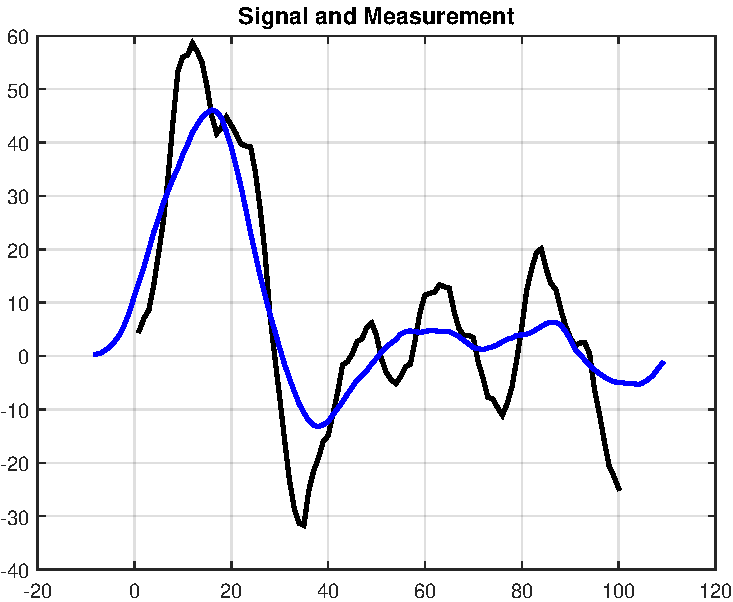
\includegraphics[width=.5\textwidth]{problem1.pdf}\end{center}

\problem{Estimation: Construct an optimal linear estimate $\hat x$ and the variance matrix $\Var(\hat x - x)$. Show on the same graph} 

  \subproblem{The original signal $x$ ( a curve with components $x_i$),}
  \subproblem{Its estimate $\hat x$ (a curve with components $\hat x_i$),}
  \subproblem{Standard deviations for the estimates $\hat x_i \big(=\sqrt{\Var(\hat x - x)_{ii}}$, can be illustrated by showing the corresponding ``corridor'' around $\hat x_i\big)$.}

\lstinputlisting[language=Matlab,firstline=39,lastline=43]{measurement_simulation.m}

\begin{center}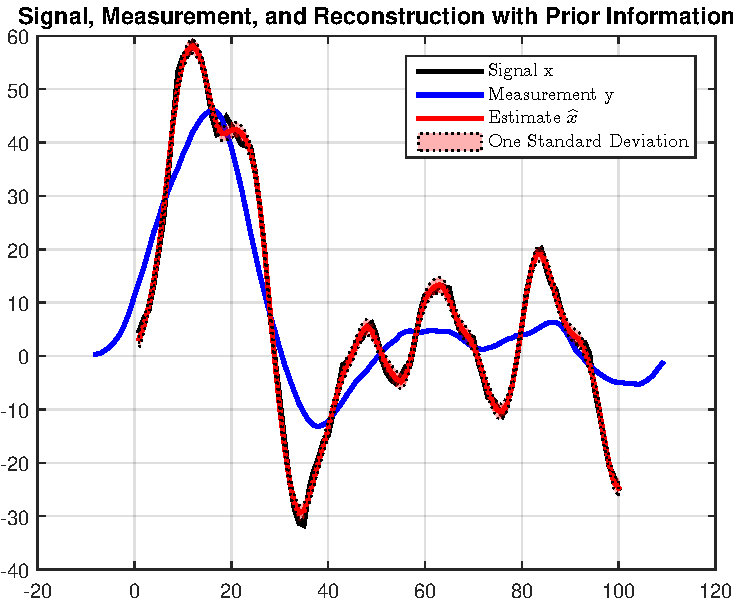
\includegraphics[width=.5\textwidth]{problem2.pdf}\end{center}

Note that the reconstruction used prior information $F$.

\problem{ Illustrate estimation (Phase 2) in different settings:}

\begin{enumerate}[(a)]
  \item Single measurement $(y,A,S)$.
  \begin{enumerate}[i.]
    \item Transform $(y,A,S)$ to canonical form $(T,v)$.
    \item Construct the estimate, based on the canonical information.
  \end{enumerate}

\lstinputlisting[language=Matlab,firstline=45,lastline=54]{measurement_simulation.m}

\begin{center}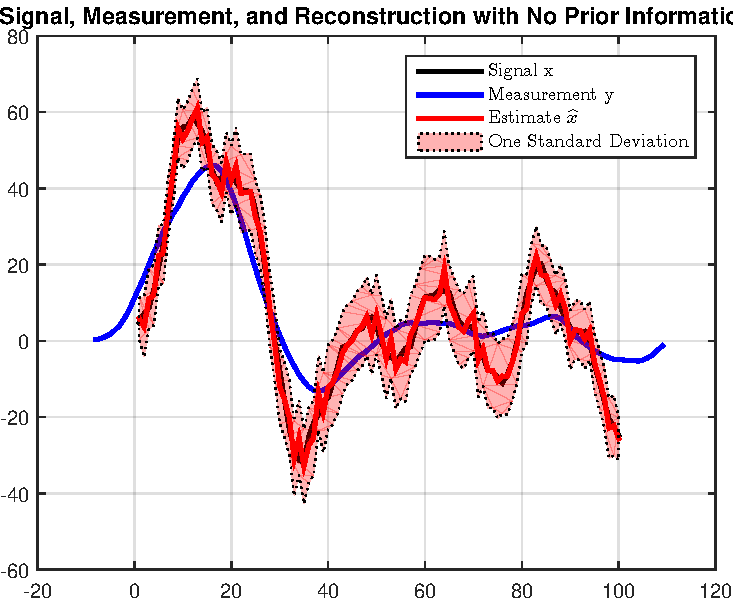
\includegraphics[width=.5\textwidth]{problem3a.pdf}\end{center}

  Observe that without prior information, there is more uncertainty in the estimate.  

  \item Single measurement $(y,A,S)$ wiht prior information: $x\sim (0,F)$.
  \begin{enumerate}[i.]
    \item Transform the measurement and the prior information to canonical form.
    \item Combine pieces of canonical information.
    \item Construct the estimate, based on the combined canonical information.
  \end{enumerate}

\lstinputlisting[language=Matlab,firstline=57,lastline=65]{measurement_simulation.m}

\begin{center}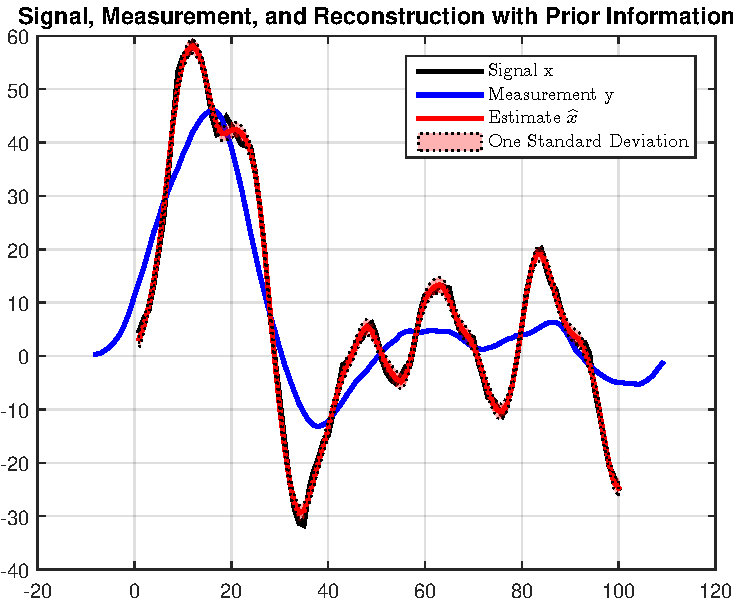
\includegraphics[width=.5\textwidth]{problem3b.pdf}\end{center}

  Note that this is precicely the same reconstruction in Problem 2.

  \item Many measurements $(y_i,A_j,S_j)$.
  \begin{enumerate}[i.]
    \item Extract canonical information from each measurement.
    \item Combine pieces of canonical information.
    \item Construct the estimate, based on the combined canonical information.
  \end{enumerate}

  The following simulates four measurements from each of the four defined blurring kernels in Problem 1. Note that in the implementation, assuming no prior information is the same as starting with an empty canonical representation. 
\lstinputlisting[language=Matlab,firstline=68,lastline=89]{measurement_simulation.m}

\begin{center}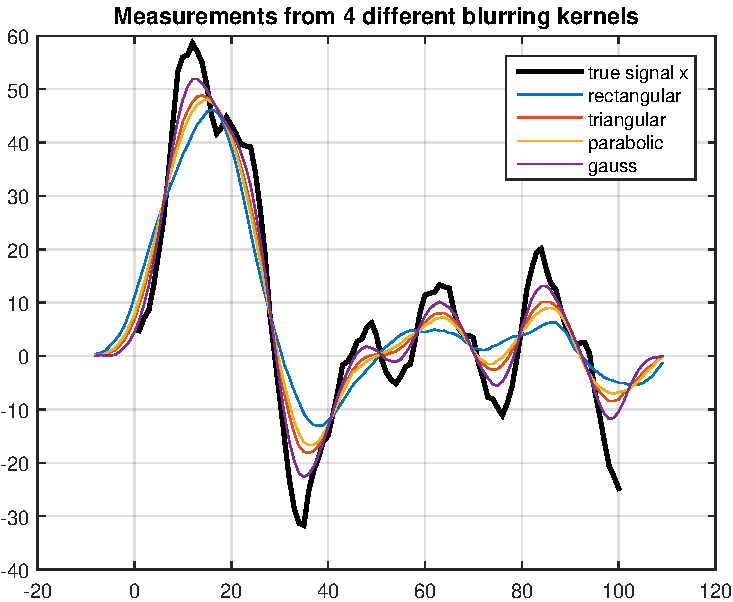
\includegraphics[width=.45\textwidth]{problem3c1.pdf}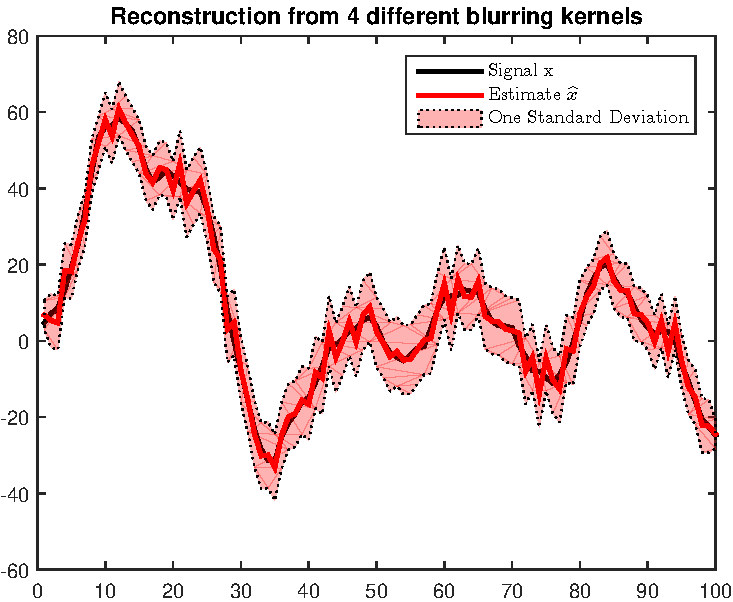
\includegraphics[width=.45\textwidth]{problem3c2.pdf}\end{center}

Observe that increasing to four measurements reduces the uncertertainty but not by much. 
If ten measurements are taken with each of the four ``devices'' ($n=40$), we see a substantial decrease in uncertainty, although not as much as including accurate prior information.

\begin{center}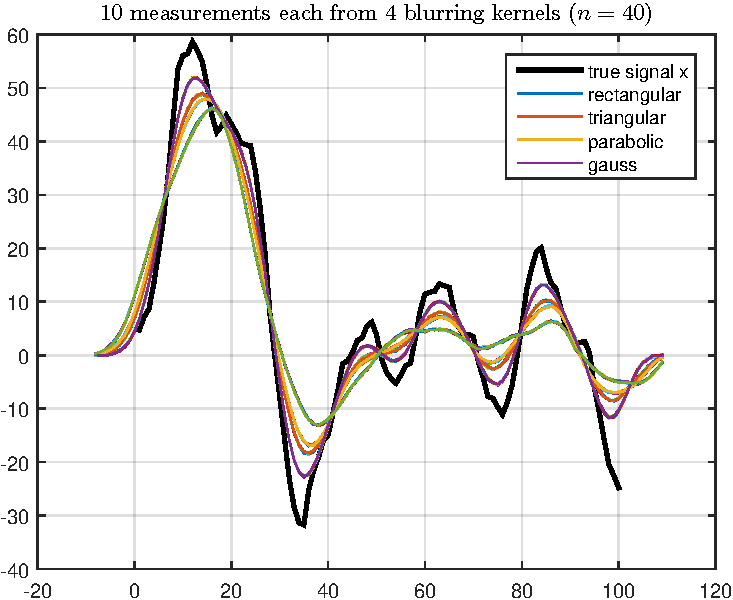
\includegraphics[width=.45\textwidth]{problem3c3.pdf}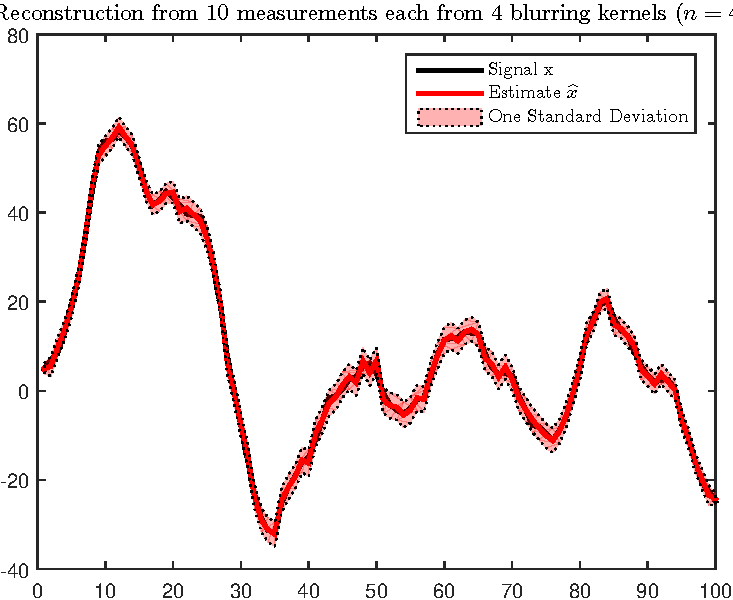
\includegraphics[width=.45\textwidth]{problem3c4.pdf}\end{center}

  \item Many measurements $(y_j,A_j,S_j)$ with a prior information $x \sim (0,F)$.  Same as item (c).

\lstinputlisting[language=Matlab,firstline=118,lastline=130]{measurement_simulation.m}

For this problem, we use the same use the same four simulated measurements from 3c. Note that the only modification to the code is that the loop now starts with the canonical representation of the prior $x \sim (0,F)$.
\begin{center}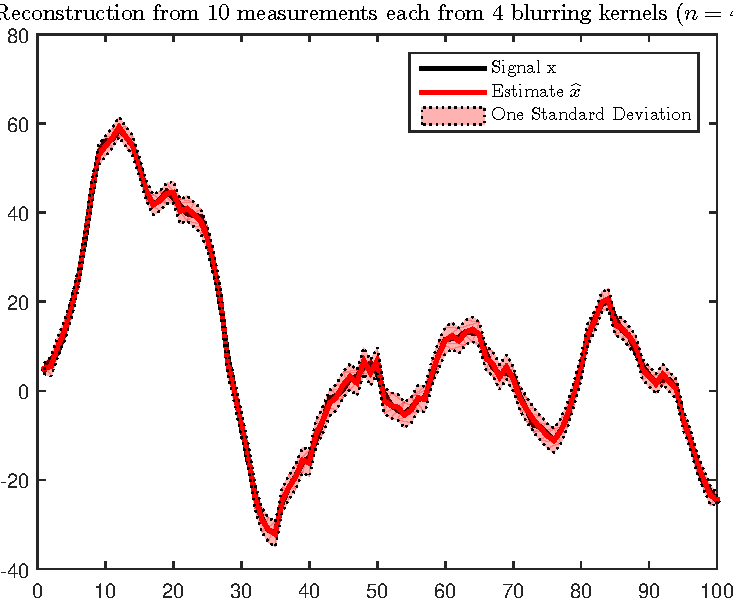
\includegraphics[width=.5\textwidth]{problem3d.pdf}\end{center}

\end{enumerate}
\end{document} 


